\setcounter{section}{0}
Vận tốc $v$ phụ thuộc thời gian theo hàm bậc nhất nên đồ thị vận tốc - thời gian có dạng là một nửa đường thẳng (do thời gian không âm) giới hạn bởi điểm ($t_0$, $x_0$). Như vậy:
\begin{itemize}
	\item Nếu gia tốc $a>0$ thì đồ thị hướng lên trên;
	\item Nếu gia tốc $a<0$ đồ thị hướng xuống dưới.
\end{itemize}
\begin{center}
	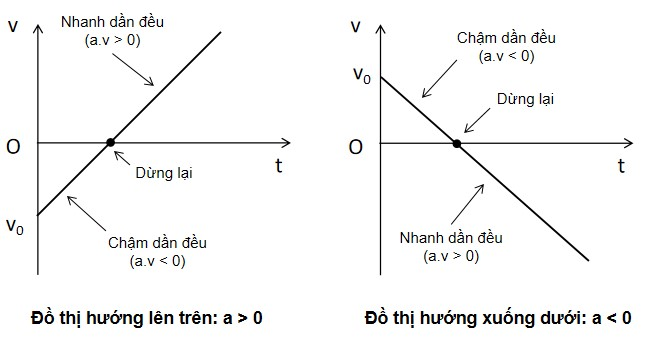
\includegraphics[scale=0.8]{../figs/VN10-PH-04-L-003-3-V2-01.jpg}
\end{center}	
\setcounter{viduii}{0}
	\viduii{3}{Đồ thị vận tốc thời gian của một vật chuyển động như hình vẽ bên.
	\begin{center}
		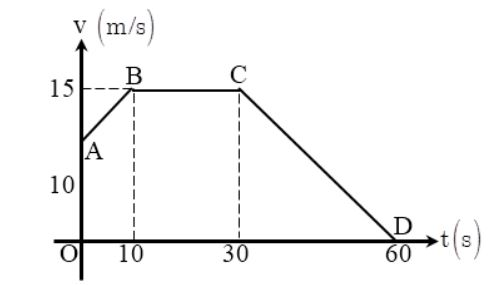
\includegraphics[scale=0.8]{../figs/VN10-PH-04-L-003-3-V2-04.jpg}
	\end{center}
	
	\begin{enumerate}
		\item Nêu tính chất chuyển động của mỗi giai đoạn.
		\item Lập phương trình vận tốc của mỗi giai đoạn.
	\end{enumerate}
	
}
{	\begin{center}
		\textbf{Hướng dẫn giải}
	\end{center}
		\begin{enumerate}
		\item Nêu tính chất chuyển động của mỗi giai đoạn.
	
	AB: chuyển động nhanh dần đều.
	
	BC: chuyển động thẳng đều.
	
	CD: chuyển động chậm dần đều.
	
			\item Lập phương trình vận tốc của mỗi giai đoạn.
	
	$$v_\text{AB} = 10 +\text{0,5}\ \text{m/s} t\ (0\leq t \leq 10).$$
	
	$$v_\text{BC} = \SI{15}{m/s}.$$
	
	$$v_\text{CD} = 15 - \text{0,5}(t-30)\ \ \text{m/s} ; (30 \leq t \leq 60).$$
\end{enumerate}
}

\begin{enumerate}[label=\bfseries Câu \arabic*:]
	\item \mkstar{3}
	
	{ Từ các đồ thị trong hình:
		\begin{center}
			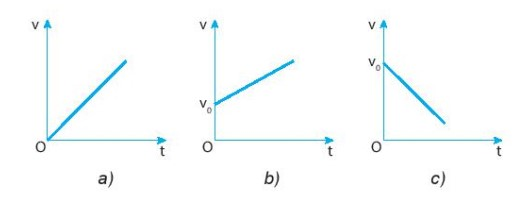
\includegraphics[scale=1]{../figs/VN10-2022-PH-TP012-1.jpg}
		\end{center}
		
		\begin{enumerate}[label=\alph*)]
			\item Hãy viết công thức về mối liên hệ giữa $v$ với $a$ và $t$ của từng chuyển động ứng với từng đồ thị trong hình.
			\item Chuyển động nào là chuyển động nhanh dần dều, chậm dần đều?
		\end{enumerate}
		
	}
	
	\hideall{
		
		\begin{enumerate}[label=\alph*)]
			\item 
			- Đồ thị a: $$v=at.$$
		
			- Đồ thị b: $$v = v_0 + at.$$
	
			- Đồ thị c: $$v = v_0 -at.$$
			\item 
			
			- Chuyển động nhanh dần đều là: đồ thị a và b.
			
			- Chuyển động chậm dần đều: đồ thị c.
			
			
			
		
		\end{enumerate}

	}
		\item \mkstar{3}
	
	{ Hãy dựa vào đồ thị để mô tả bằng lời chuyển động của bạn đó khi đi siêu thị (khi nào đi đều, đi nhanh lên, đi chậm lại, nghỉ).
		\begin{center}
			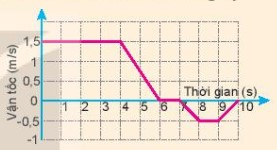
\includegraphics[scale=1]{../figs/VN10-2022-PH-TP012-2.jpg}
		\end{center}
		
	}
	
	\hideall{
		
		- Trong 4 s đầu tiên: bạn đó đi đều với vận tốc $\SI{1,5}{m/s}$.
		
		- Từ giây 4 – giây 6: bạn đó đi chậm lại.
		
		- Từ giây 6 đến giây 7: bạn đó nghỉ.
		
		- Từ giây 7 đến giây 8: bạn đó bắt đầu đi theo chiều âm.
		
		- Từ giây 8 – 9: bạn đó đi đều với vận tốc $-\SI{0,5}{m/s}$.
		
		- Từ giây 9 – 10: đi chậm và dừng lại tại giây thứ 10.
		
	}
		\item \mkstar{3}
	
	{Hãy tính độ dịch chuyển của chuyển động có đồ thị ($v - t$) vẽ ở hình. Biết mỗi cạnh của ô vuông nhỏ trên trục tung ứng với $\SI{2}{m/s}$, trên trục hoành ứng với $\SI{1}{s}$.
		\begin{center}
			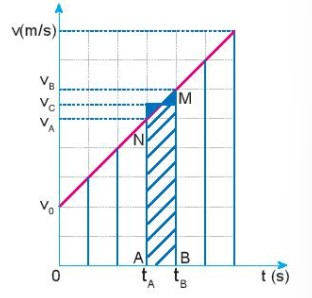
\includegraphics[scale=1]{../figs/VN10-2022-PH-TP012-3.jpg}
		\end{center}
	}
	
	\hideall{
		
		Độ dịch chuyển có độ lớn bằng diện tích của hình thang vuông có đường cao là $t$ và các đáy có độ lớn $v_0$, $v$.
		
		Từ đồ thị ta có:
		
		$$\begin{cases}
			v_0 = \SI{4}{m/s}; v = \SI{16}{m/s}.\\
			t = \SI{6}{s}.
		\end{cases}$$
		
		Độ dịch chuyển là
		
		$$d = \dfrac{(4+16)6}{2} = \SI{60}{m}.$$
	}
	
	\item \mkstar{3}

	
	{Hãy dùng đồ thị $(v-t)$ vẽ ở hình để mô tả chuyển động.
		\begin{center}
			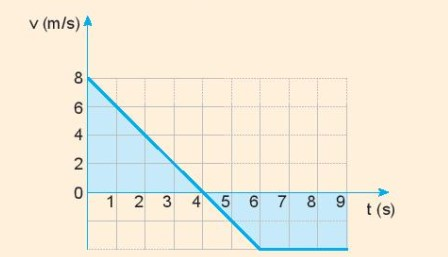
\includegraphics[scale=1]{../figs/VN10-2022-PH-TP012-4.jpg}
		\end{center}
	}

	\hideall
	{	
		- Trong 4 giây đầu tiên: chuyển động chậm dần đều từ  $\SI{8}{m/s}$ đến  $\SI{0}{m/s}$.
		
		- Từ giây thứ 4 đến giây thứ 6: bắt đầu tăng tốc với vận tốc  $- \SI{2}{m/s}$.
		
		- Từ giây thứ 6 đến giây thứ 9: chuyển động thẳng đều với vận tốc $- \SI{2}{m/s}$.
		
	}
	\item \mkstar{3}

	
	{Hãy dùng đồ thị $(v-t)$ vẽ ở hình để tính độ dịch chuyển trong 4 giây đầu, 2 giây tiếp theo và 3 giây cuối.
		\begin{center}
			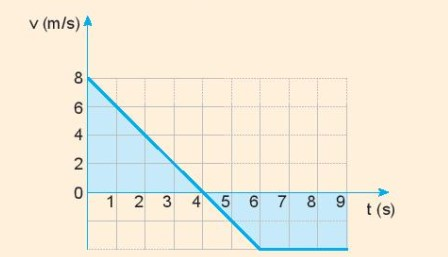
\includegraphics[scale=1]{../figs/VN10-2022-PH-TP012-4.jpg}
		\end{center}
	}

	\hideall
	{
		- Trong 4 giây đầu:
		
		Độ dịch chuyển bằng diện tích tam giác vuông có cạnh đáy là $t$ và chiều cao là $v$.
		
		$$d_1 = \dfrac{1}{2}v_1t_1 = \SI{16}{m}.$$
		
		- Trong 2 giây tiếp theo:
		
		Độ dịch chuyển bằng diện tích tam giác vuông có cạnh đáy là $t$ và chiều cao là $v$.
		
		$$d_2 = \dfrac{1}{2}v_2t_2 = -\SI{4}{m}.$$
		
		- Trong 3 giây cuối:
		
		Độ dịch cuyển bằng diện tích hình chữ nhật có chiều dài là $t$ và chiều rộng là $v$.
		
		$$d_3 = \dfrac{1}{2}v_3t_3 = -\SI{12}{m}.$$
		
		
	}
	\item \mkstar{3}

	
	{
		Hãy dùng đồ thị $(v-t)$ vẽ ở hình để tính gia tốc của chuyển động trong 4 giây đầu.
		\begin{center}
			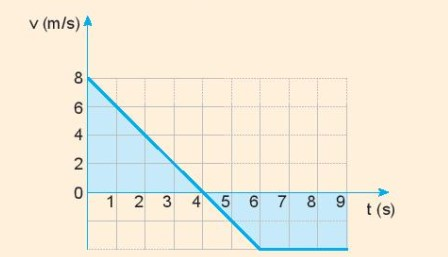
\includegraphics[scale=1]{../figs/VN10-2022-PH-TP012-4.jpg}
		\end{center}
	}

	\hideall
	{	
		Gia tốc của chuyển động trong 4 giây đầu
		
		$$a = \dfrac{\Delta v}{\Delta t} =\dfrac{8 - 0}{4-0}= \SI{2}{m/s}^2.$$
	}
	\item \mkstar{4}

	
	{Hãy dùng đồ thị $(v-t)$ vẽ ở hình để tính gia tốc của chuyển động từ giây thứ 4 đến giây thứ 6.
		\begin{center}
			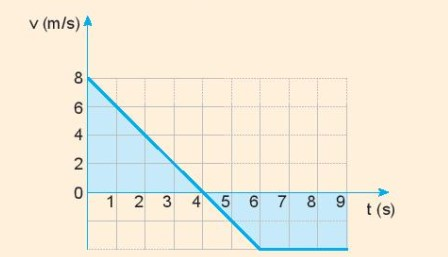
\includegraphics[scale=1]{../figs/VN10-2022-PH-TP012-4.jpg}
		\end{center}
	}

	\hideall
	{	
		Gia tốc của chuyển động từ giây thứ 4 đến giây thứ 6:
		
		$$a = \dfrac{\Delta v}{\Delta t} =\dfrac{-4 - 0}{6-4}= -\SI{2}{m/s}^2.$$ 
	}
	\item \mkstar{4}

	
	{Đồ thị vận tốc - thời gian ở hình mô tả chuyển động của một chú chó con đang chạy trong một ngõ thẳng và hẹp.
		\begin{center}
			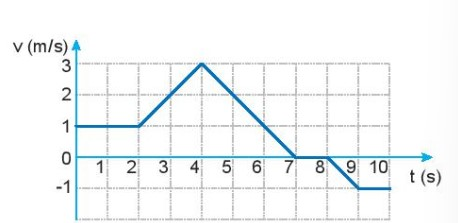
\includegraphics[scale=1]{../figs/VN10-2022-PH-TP012-5.jpg}
		\end{center}
		
		\begin{enumerate}[label=\alph*)]
			\item Hãy mô tả chuyển động của chú chó.
			\item Tính quãng đường đi được và độ dịch chuyển của chú chó sau $\SI{2}{s}$; $\SI{4}{s}$; $\SI{7}{s}$ và $\SI{10}{s}$ bằng đồ thị.
		\end{enumerate}
	}

	\hideall
	{	
		\begin{enumerate}[label=\alph*)]
			\item 
			- Trong 2 giây đầu tiên: chuyển động thẳng đều với vận tốc $\SI{1}{m/s}$.
			
			- Từ giây thứ 2 đến giây thứ 4: chuyển động nhanh dần đều.
			
			- Từ giây 4 đến giây 7: chuyển động chậm dần.
			
			- Từ giây 4 đến giây 8: dừng lại.
			
			- Từ giây 8 đến giây 9: chuyển động nhanh dần theo chiều âm.
			
			- Từ giây 9 đến giây 10 chuyển động thẳng đều với vận tốc $-\SI{1}{m/s}$.
			
		
			\item 
			- Sau 2 giây:
			
			$$s_1 = d_1 = v_1 t_1 = \SI{2}{m/s}.$$
			
			- Sau 4 giây:
			
			$$s_2 = d_2 = s_1 + \dfrac{1}{2} (1+3)2 = \SI{6}{m}.$$
			
			- Sau 7 giây:
			
			+ Quãng đường:
			
			$$s_3 = s_2 + \dfrac{1}{2} (7-4)3 = \SI{10,5}{m}.$$
			
			+ Độ dịch chuyển:
			
			$$d_3 = d_2 + \dfrac{1}{2} (7-4)3 = \SI{10,5}{m}.$$
			
			- Sau 10 giây:
			
			+ Quãng đường:
			
			 Từ giây 7 – 8: đứng yên
		
			$$s_4 = s_3 + s' = \text{10,5} + \text{0,5} + 1 = \SI{12}{m}.$$
			
			+ Độ dịch chuyển:
			
			$$d_4 = d_3 + d' = \text{10,5} - \text{0,5} - 1 = \SI{9}{m}.$$
			
		\end{enumerate}
	}
	\item \mkstar{4}

	
	{Một vận động viên đua xe đạp đường dài vượt qua vạch đích với vận tốc $\SI{10}{m/s}$. Sau đó vận động viên này đi chậm dần đều thêm $\SI{20}{m}$ mới dừng lại. Coi chuyển động của vận động viên là thẳng.
		\begin{enumerate}[label=\alph*)]
			\item Tính gia tốc của vận động viên trong đoạn đường sau khi qua vạch đích.
			\item Tính thời gian vận động viên đó cần để dừng lại kể từ khi cán đích.
			\item Tính vận tốc trung bình của người đó trên quãng đường dừng xe.
		\end{enumerate}
	}

	\hideall
	{	
		\begin{enumerate}[label=\alph*)]
			\item Gia tốc của vận động viên trong đoạn đường sau khi qua vạch đích
			
			$$v^2 - v_0^2 = 2ad \Rightarrow a = -\SI{2,5}{m/s}^2.$$
			
			\item Thời gian vận động viên đó cần để dừng lại kể từ khi cán đích
			
			$$a = \dfrac{\Delta v}{\Delta t} \Rightarrow  \Delta t = \SI{4}{s}.$$
			 
			\item Vận tốc trung bình của người đó trên quãng đường dừng xe
			
			$$v = \dfrac{d}{t} = \SI{5}{m/s}.$$
		\end{enumerate}
	}
	\item \mkstar{4}

	
	{Hình biểu diễn đồ thị vận tốc - thời gian của một quả bóng thả rơi chạm đất rồi nảy lên theo phương thẳng đứng. Quả bóng được thả tại A và chạm đất tại B. Quả bóng rời khỏi mặt đất tại D và đạt độ cao cực đại tại E. Có thể bỏ qua tác dụng của lực cản không khí.
		\begin{center}
			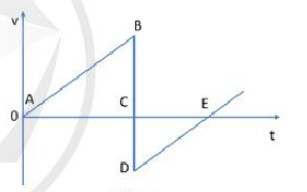
\includegraphics[scale=1]{../figs/VN10-2022-PH-TP012-6.jpg}
		\end{center}
		
		\begin{enumerate}[label=\alph*)]
			\item Tại sao độ dốc của đoạn thẳng AB lại giống độ dốc của đoạn thẳng DE?
			\item Diện tích tam giác ABC biểu thị đại lượng nào?
			\item Tại sao diện tích tam giác ABC lớn hơn diện tích tam giác CDE?
		\end{enumerate}
	}

	\hideall
	{	
		\begin{enumerate}[label=\alph*)]
			\item - Độ dốc của đường thẳng có giá trị bằng gia tốc.
			
			- AB và DE đều là đường thẳng nên gia tốc không đổi, vì vậy độ dốc của đoạn thẳng AB giống độ dốc của đoạn thẳng DE.
			
			
			\item Diện tích tam giác ABC biểu diễn quãng đường dịch chuyển của quả bóng từ A đến B.
			
			
			\item - Diện tích tam giác ABC biểu diễn quãng đường dịch chuyển của vật từ A đến B.
			
			- Diện tích tam giác CDE biểu diễn quãng đường dịch chuyển của vật từ D đến E.
			
			- Trong quá trình chuyển động của quả bóng thì cơ năng được bảo toàn, nhưng khi quả bóng đi từ A đến B thì năng lượng của quả bóng bị mất đi do một phần bị tỏa nhiệt, vì vậy năng lượng của quả bóng giảm đi nên khi quả bóng đi từ D đến E thì quãng đường DE ngắn hơn quãng đường AB. Vì vậy diện tích tam giác ABC lớn hơn diện tích tam giác CDE.
			
			
		\end{enumerate}
	}
\end{enumerate}